\documentclass{article}
\usepackage{amsmath,amssymb,stmaryrd}
\usepackage[margin=1in]{geometry}
\usepackage{graphicx}

\title{Learning Communication, Coalgebraically}
\author{}
\date{}

\begin{document}
\maketitle

\section{The question}

How can two agents learn to communicate?

Imagine a sequential interaction in which each of two players can output messages, but these messages may initially be written in completely different \emph{languages} (or even modalities).
How, in principle, can they bridge this gap and eventually communicate?

One response would be to create some external goal that the two players must mutually achieve and to treat language like any other action to be reinforcement-learned. Specifically, a particular elegant and instrumentally convergent task is that of predicting future observations. 

At this point, there are several modelling choices.
For instance, we could give A access to B's next observation and have A learn to give short messages to B such that B can predict its observations conditional on A's messages (the messages would have to be short or of a different type as the observations to be interesting, because otherwise the message could be a copy of the observations).

\bigskip
\begin{center}
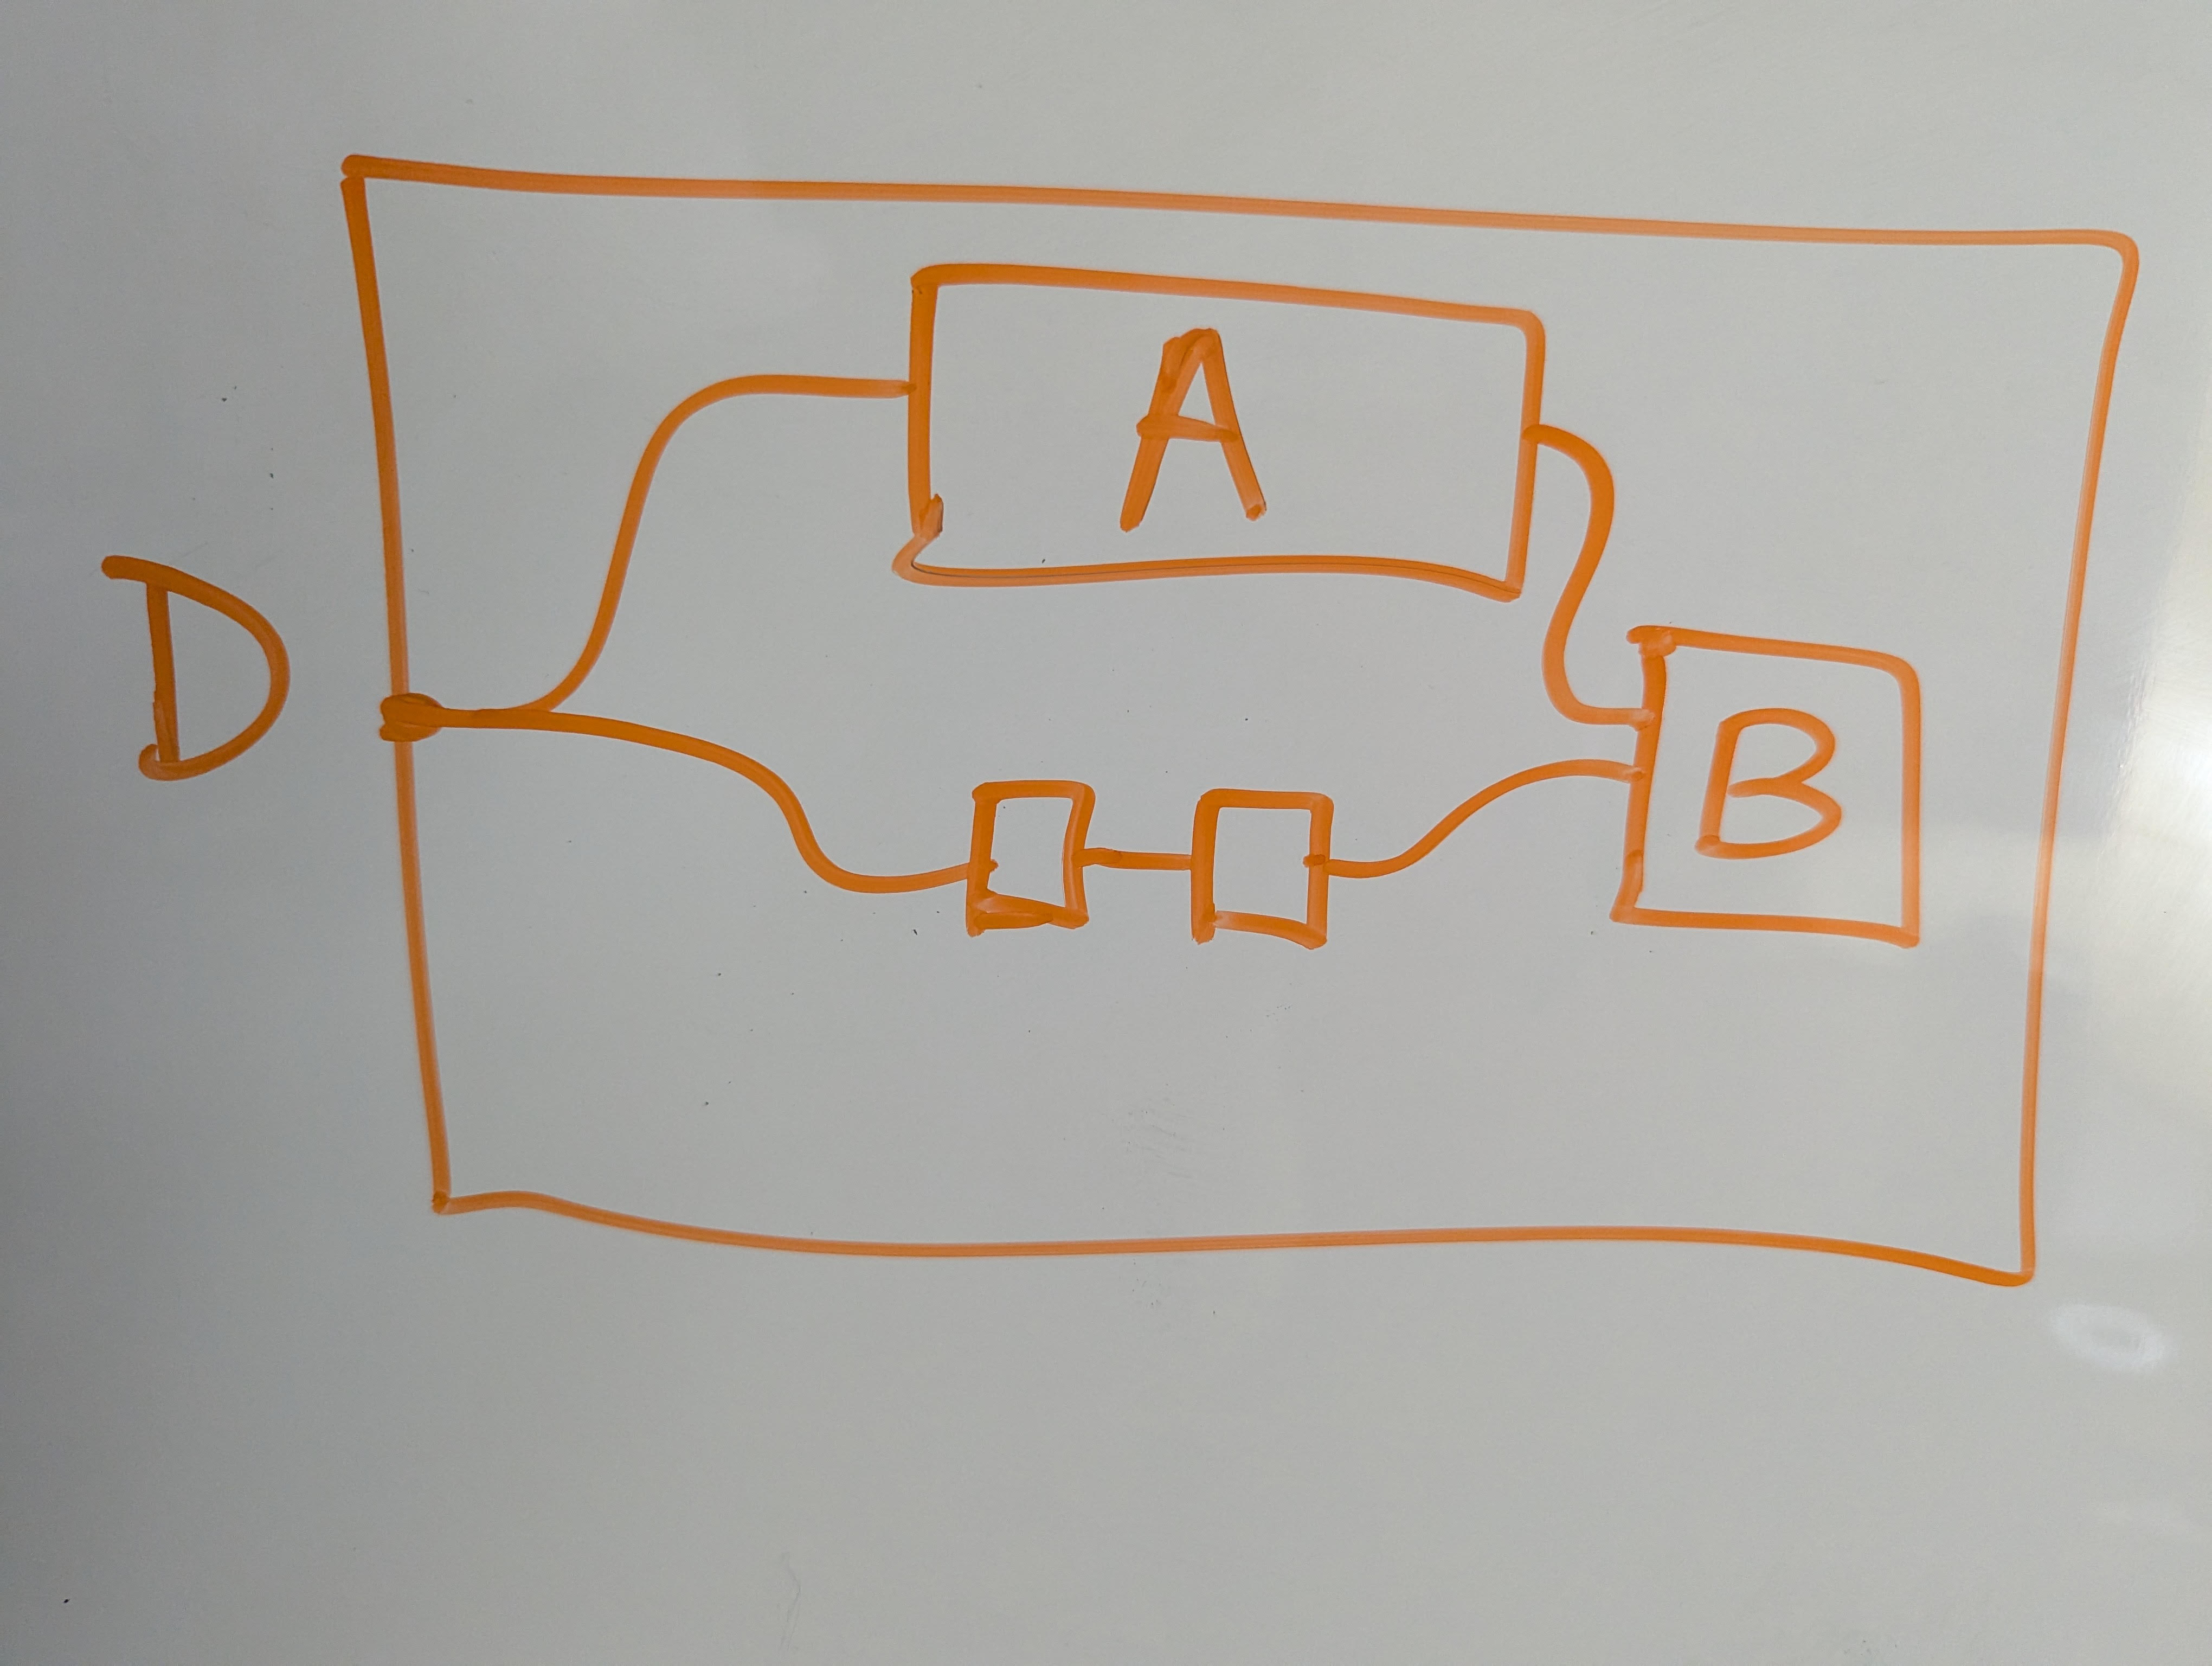
\includegraphics[width=0.3\textwidth]{Apriority.jpg}
\end{center}

\section{Toward a symmetric setup}

But this setup eschews some of the more cooperative/bidirectional/mutually recursive aspects of the genesis of effective communication.
Instead, consider a situation where neither player has privileged information to incoming data; rather they both have access to a shared input data stream. They each can send messages to the other player, and each player's goal is to maximize the sum of the log probabilities that each player ascribes to their observations, making it a kind of cooperative game.

$$
\lim_{T \to \infty} \frac{1}{T} \sum_{t=1}^{T} \left( \log P_A(\text{observation}_t) + \log P_B(\text{observation}_t) \right)
$$

\bigskip

\begin{center}
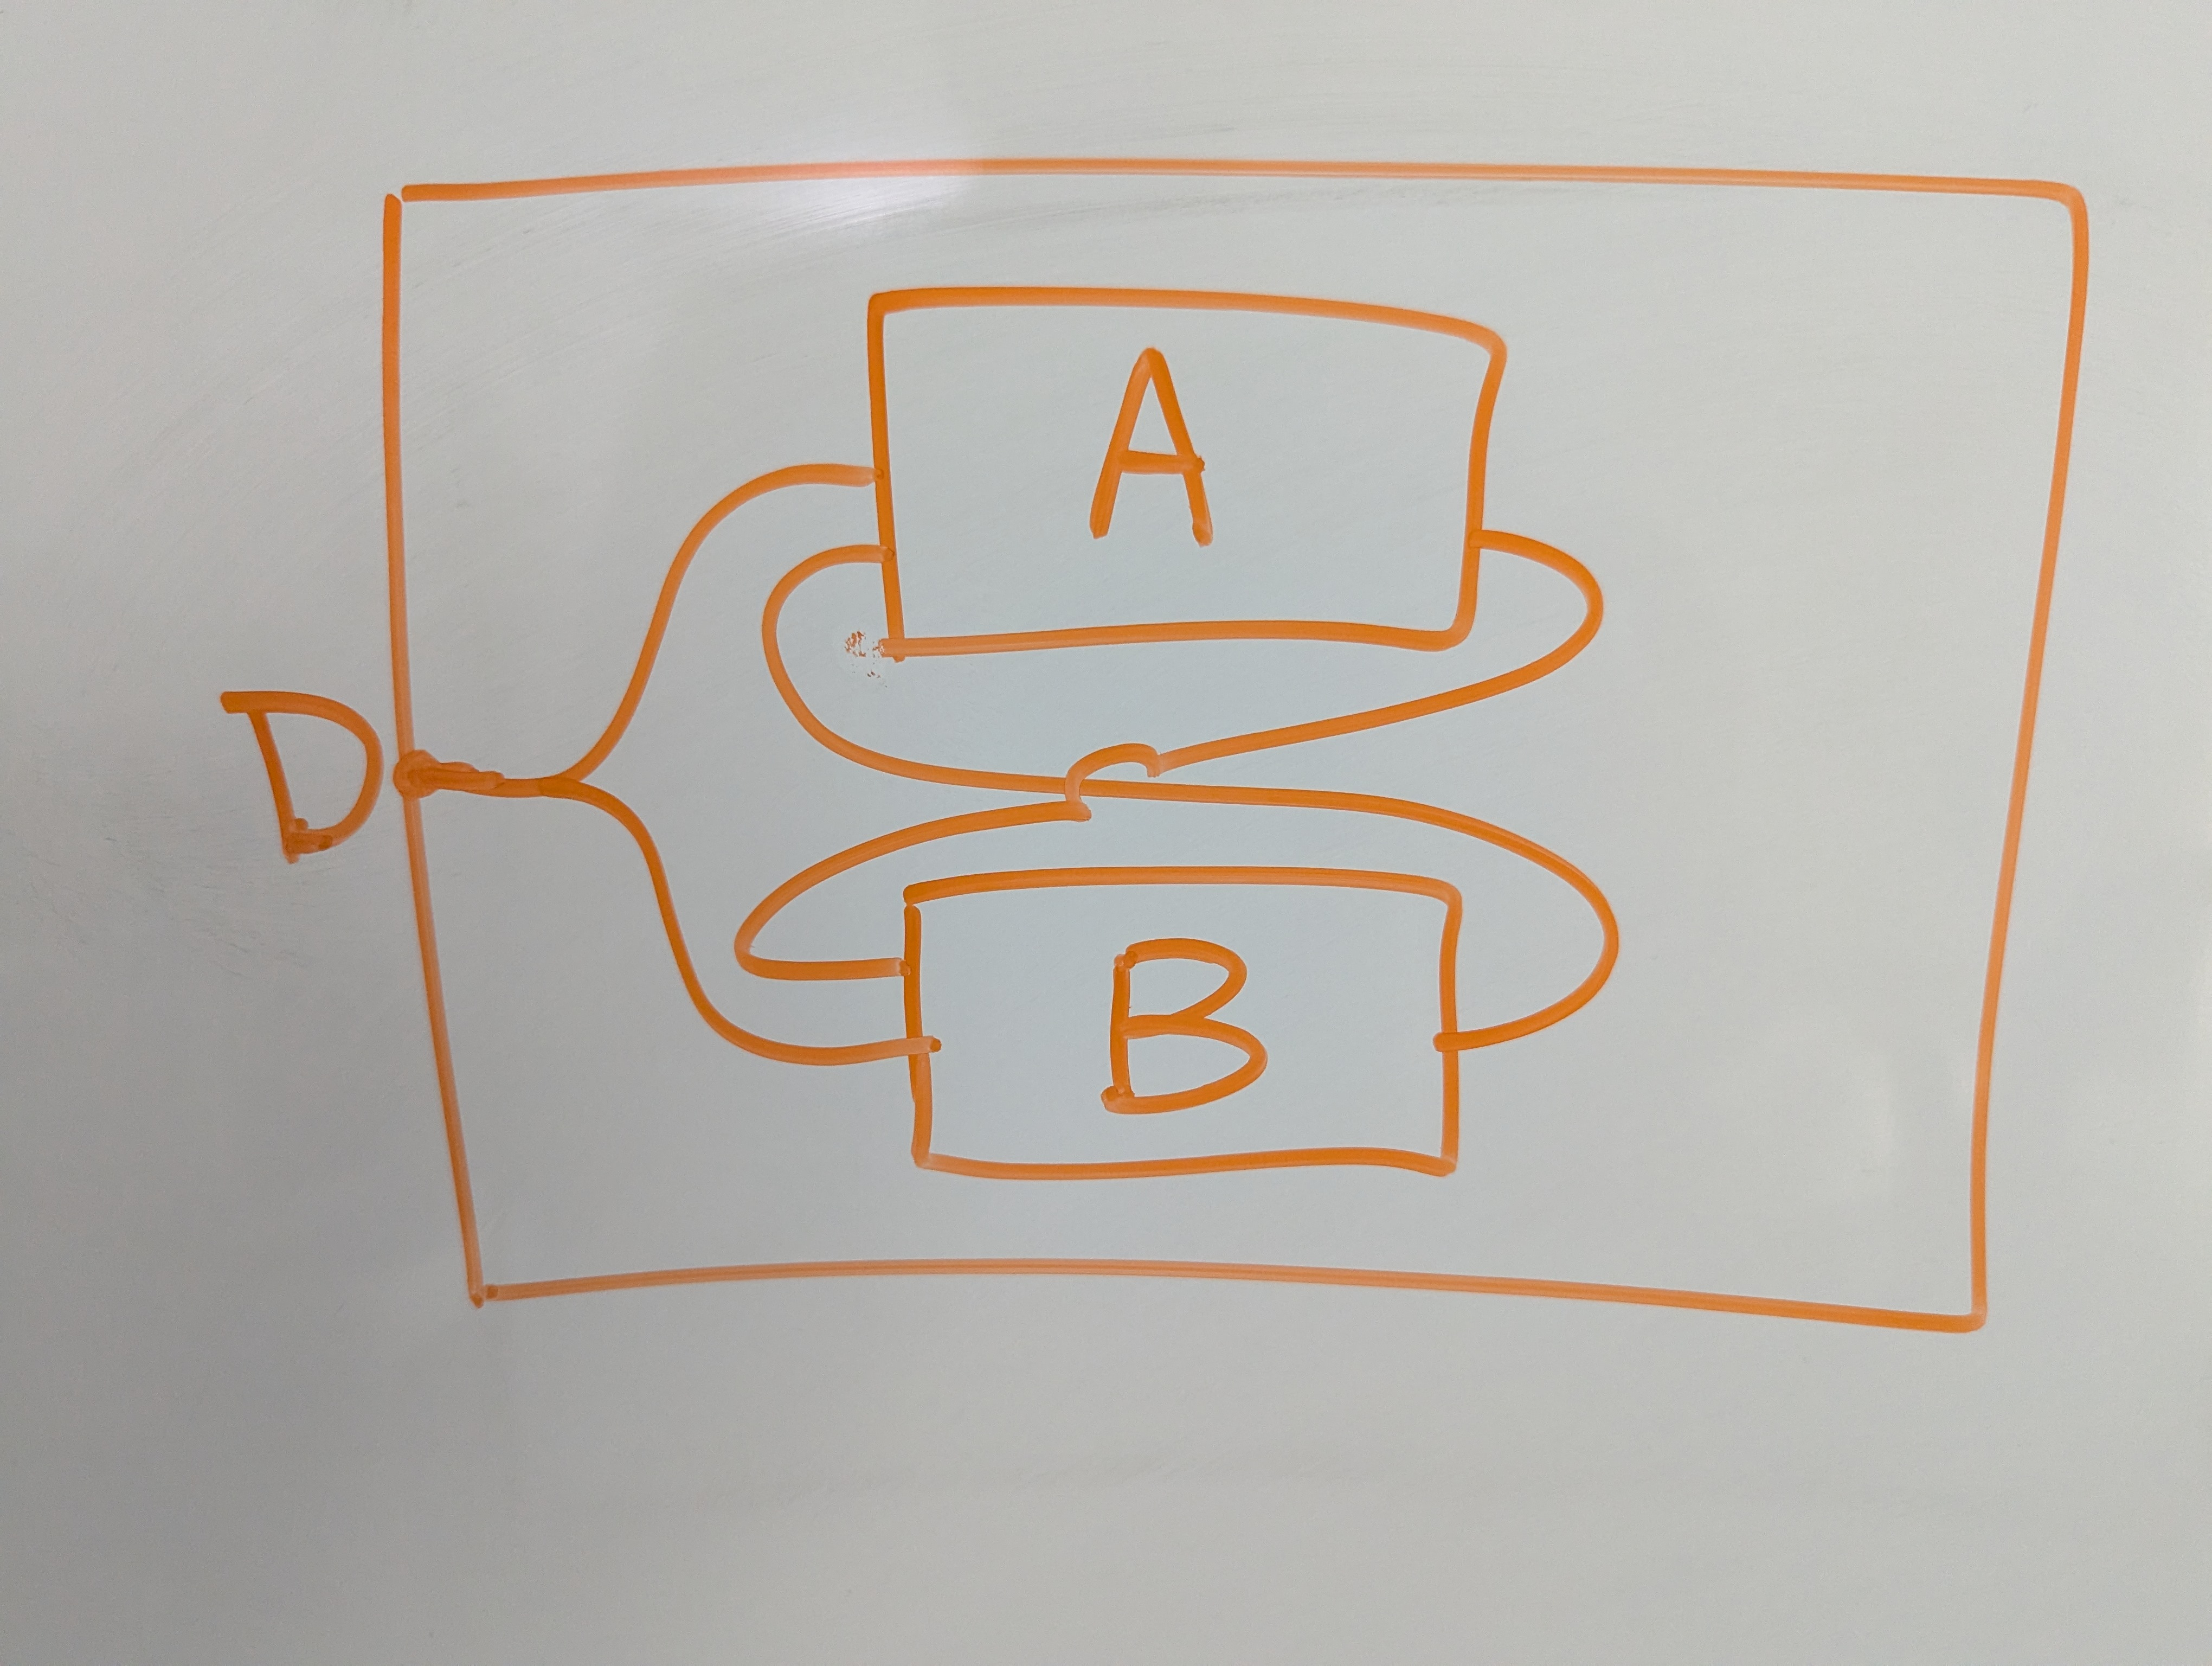
\includegraphics[width=0.3\textwidth]{simple.jpg}
\end{center}

\section{Players as coalgebras}

We can model each player then as an $F$-coalgebra 
$(S_X,\;\alpha_X\colon S_X\longrightarrow F S_X)$,where $F$ will be specialized to encode the notion that a player can \emph{receive inputs} and \emph{produce outputs} -- e.g. $F(S)\;=\;\mathsf{Out}\times S^{\mathsf{In}}$ for some types $\mathsf{Out}$ and $\mathsf{In}$.

Now we can add in requirements on the structure of $S$, $\mathsf{Out}$, and $\mathsf{Out}$ to match the problem setup. First, to model the emergence of communication, we should model the ability of the players to learn. We can do this by expressing $S$ as $\Theta \times \_$, where $\Theta$ is the space of parameterizations of the player's behavior. Next $\mathsf{Out}$ must include A's ``raw'' message type $M_{A\rightarrow B}$. It is ``raw'' because we will need to include some metadata in order to give the learning algorithm the necessary reward signals. 

Next we have $\mathsf{In}_A$ and $\mathsf{In}_B$ which each consist of the other player's output type and the data type $D$ to be predicted: $\mathsf{In}_A=\mathsf{Out}_B \times D$ and $\mathsf{In}_B=\mathsf{Out}_A \times D$.

Then we need a way of talking about the ``probability that a player ascribes to an observation'', and for the learning algorithm to work we will also need to compute the ``probability of taking a particular action'', where both of these functions are parameterized by $\theta \in \Theta$.
$$
\Theta \xrightarrow{\pi, P} (\Delta M)(\Delta D)^M
$$ where $\pi$ is called the policy, and we require implementations of $\pi$ and $P$ for both players. So the policy produces a distribution over output messages (actions) given a state, and the predictive model $P$ produces a function from messages to distributions over input data.

The state update part of $\alpha$ is going to be a gradient descent step with respect to $\theta \in \Theta$, but the loss function needs to include not only a player A's own score $\ln P_\theta^A(d \mid m_{B \rightarrow A})$, but also B's score from the previous round given A's previous message.

So A's state must include not just their weights $\theta_A \in \Theta_A$, but also the score that B received in the previous timestep as well as the message which caused that score in the other player.
\section{Prediction and policy components}

Written out, we have $S_A = \Theta_A \times \mathbb{R} \times M_{B\rightarrow A}$ and $S_B = \Theta_B \times \mathbb{R} \times M_{A \rightarrow B}$.
Each player X consists of an initial state $s_0^X$ and functions $U_X : \mathsf{In}_X \times S_X \rightarrow S_X$ and $\Pi_X : S_X \rightarrow \mathsf{Out}_X$, where $\mathsf{Out}_A = M_{A \rightarrow B} \times \mathbb{R} \times M_{B \rightarrow A}$, $\mathsf{In}_A = D \times \mathsf{Out}_B$, and $\mathsf{In}_B = D \times \mathsf{Out}_A$.

Recall we have access to functions $\pi_A : \Theta_A \rightarrow \Delta M_{A \rightarrow B}$, $\pi_B : \Theta_B \rightarrow \Delta M_{B \rightarrow A}$, $P_A : M_{B \rightarrow A} \rightarrow \Delta D$, and $P_B : M_{A \rightarrow B} \rightarrow \Delta D$ to implement $U_A$, $U_B$, $\Pi_A$, and $\Pi_B$.

A natural choice is the following:
\begin{align*}
U_B((d, (m_{A\rightarrow B}, &r_A, m_{B \rightarrow A}^{\text{old}})) : \mathsf{In}_B, (\theta_B, \_, \_) : \Theta_B \mathbb{R} M_{A \rightarrow B}) : \Theta_B \mathbb{R} M_{A \rightarrow B} := \\
&\quad (\theta_B - \nabla_{\theta_B} \ln P_{\theta_B} (d | m_{A \rightarrow B}) - r_A \nabla_{\theta_B} \pi_{\theta_B} (m_{B \rightarrow A}^{\text{old}}), \ln P_{\theta_B} (d \mid m_{A \rightarrow B}), m_{A \rightarrow B})
\end{align*}

$$\Pi_B((\theta_B, r_B, m_{A \rightarrow B}) : S_B) : M_{B \rightarrow A} \mathbb{R} M_{A \rightarrow B} := \text{let } m_{B \rightarrow A} \sim \pi_{\theta_B}(\cdot) \text{ in } (m_{B \rightarrow A}, r_B, m_{A \rightarrow B})$$

\begin{center}
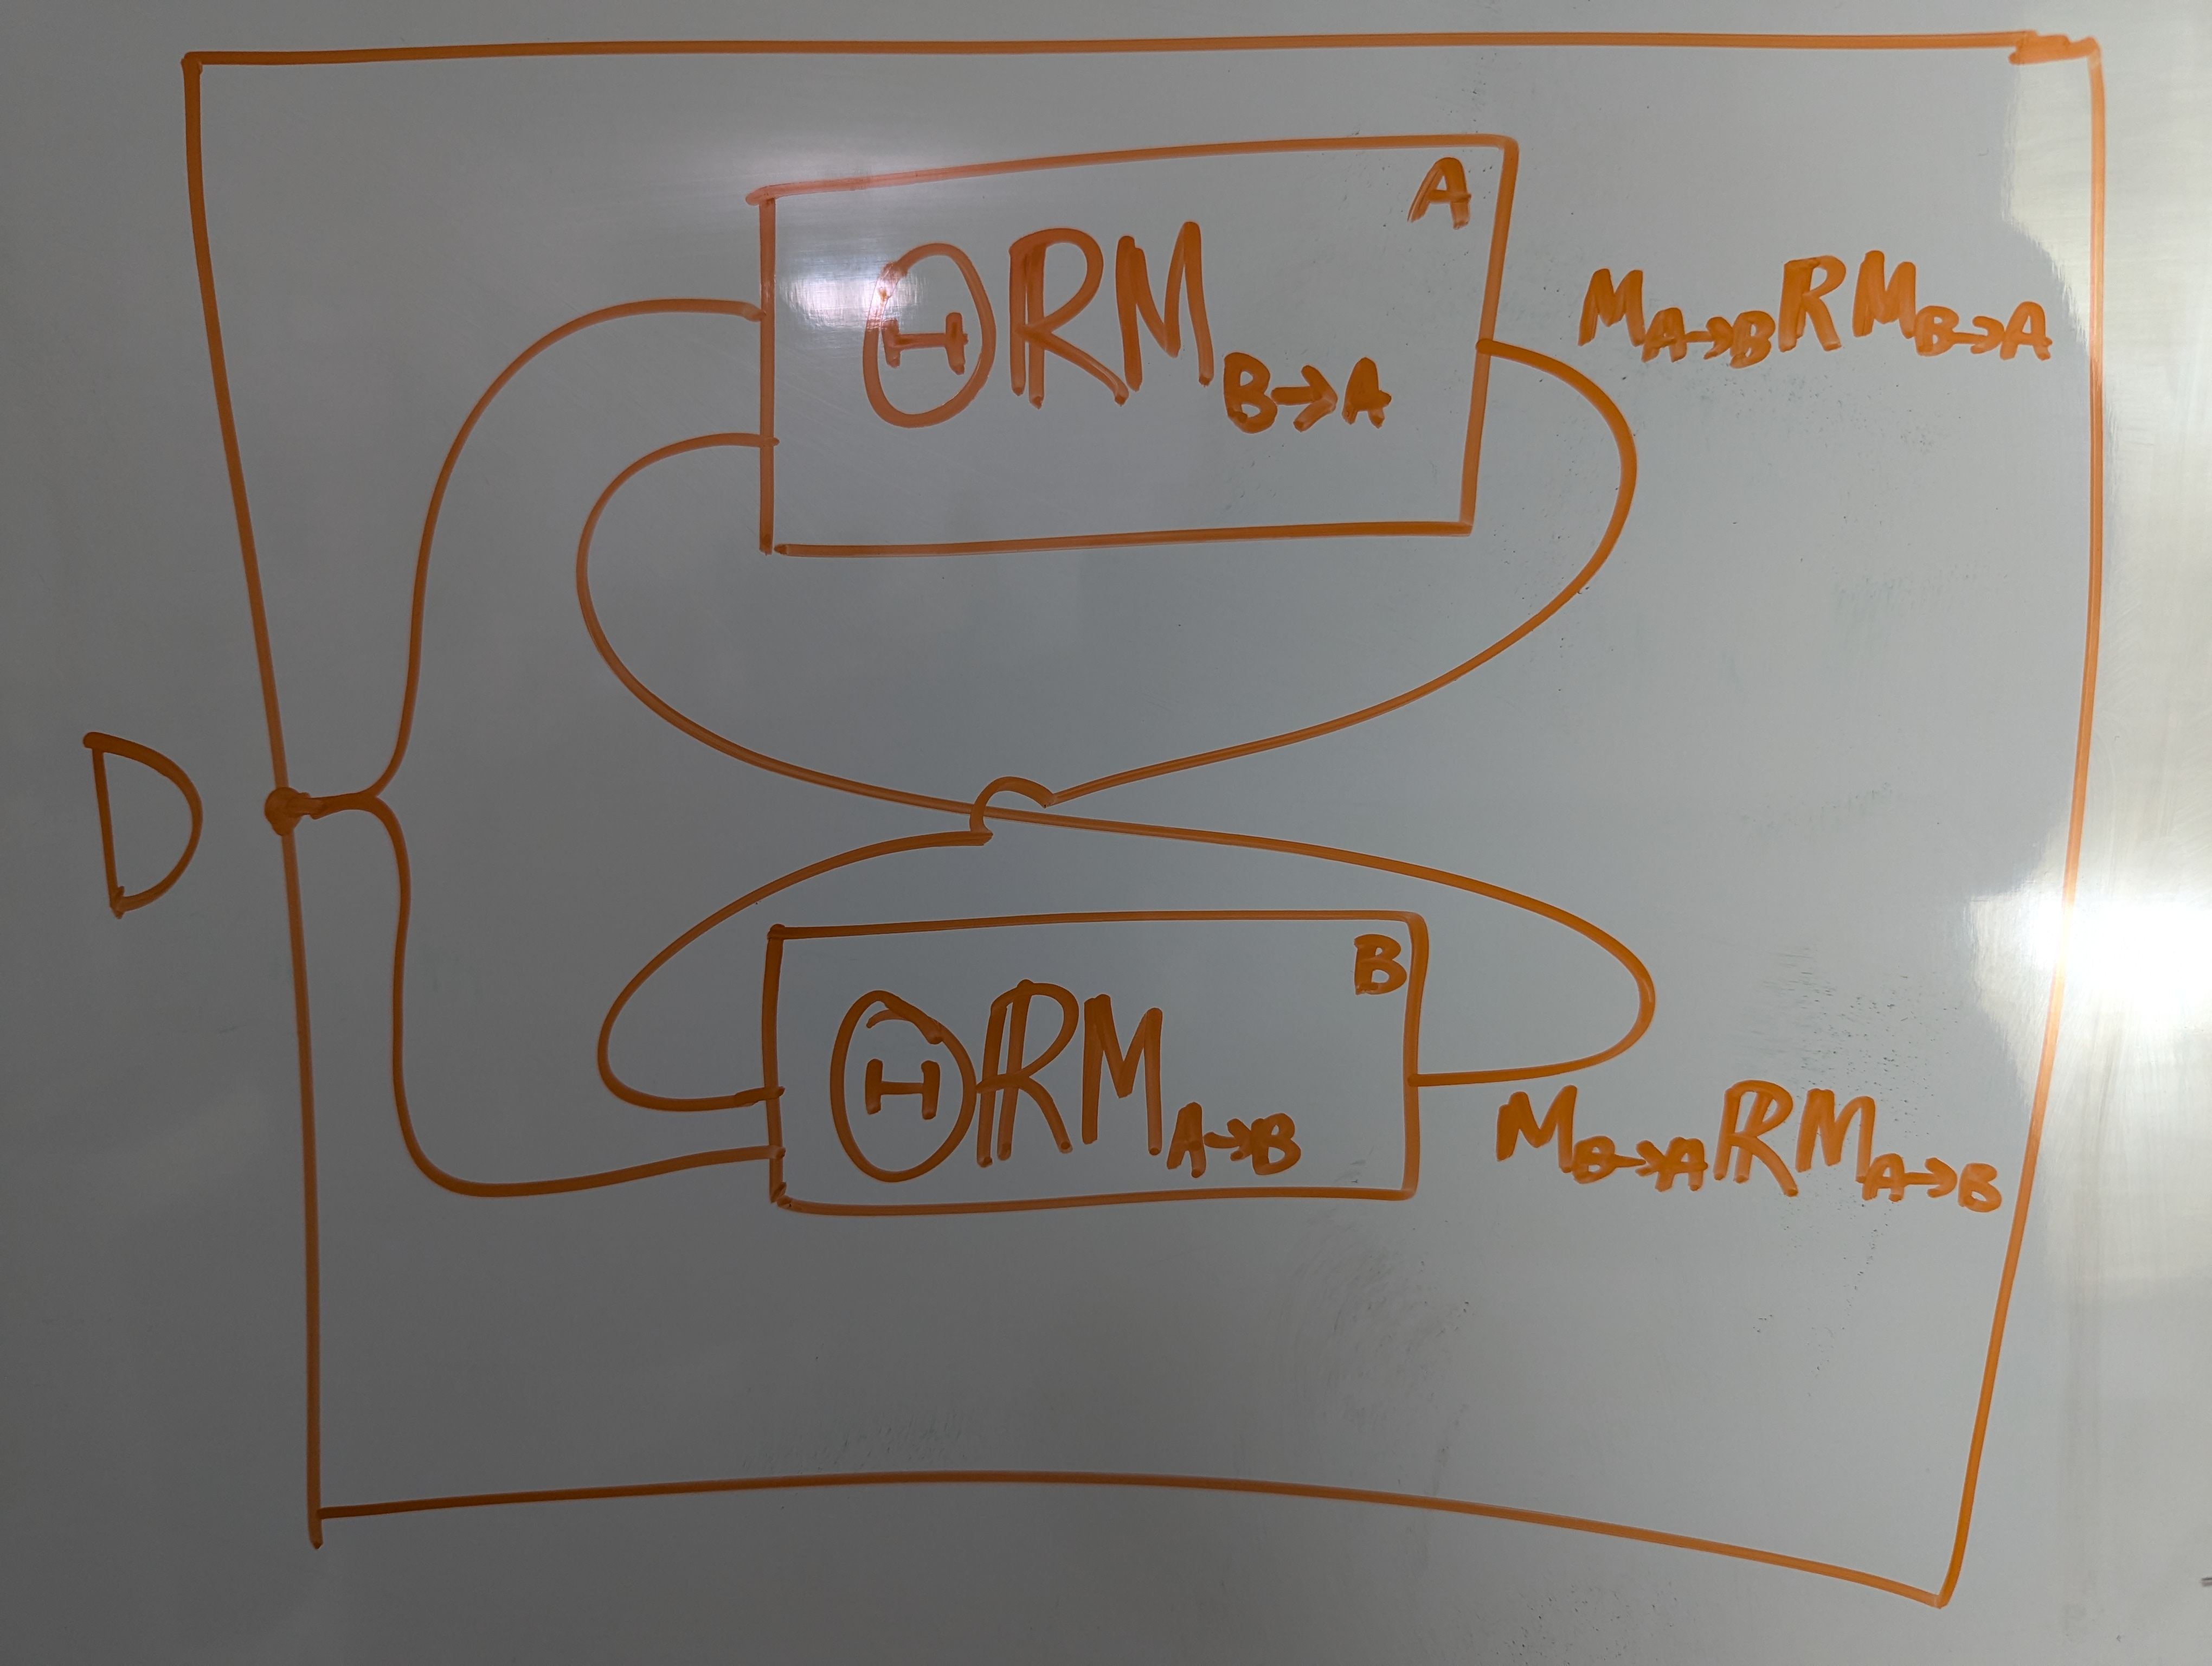
\includegraphics[width=0.5\textwidth]{detailed.jpg}
\end{center}

The important point is how the weights get updated in $U_A$ / $U_B$.
The $\nabla_{\theta_B} \ln P_{\theta_B}(d \mid m_{A \rightarrow B})$ term allows the player to get better at predicting observations given the other's messages, and $r_A \nabla_{\theta_B} (m_{B \rightarrow A})$ is a policy gradient/REINFORCE style loss term which is derived from the following observation.

\paragraph{Policy Gradient}

Given system trajectories $\tau$ distributed as $P_\theta(\tau)$, define expected reward

$$
J(\theta)=\mathbb{E}_{\tau\sim P_\theta}[R(\tau)] .
$$

Standard calculus yields

$$
\nabla_\theta J(\theta)
\;=\;
\mathbb{E}_{\tau\sim P_\theta}\!\bigl[R(\tau)\,\nabla_\theta\ln P_\theta(\tau)\bigr].
$$

Here we take

$$
R(\tau)=\frac{1}{n}\sum_{i=1}^{n}\!
\bigl(
\ln P_{\theta_B}(d_i\mid m_{A\to B}^i)
+
\ln P_{\theta_A}(d_i\mid m_{B\to A}^i)
\bigr).
$$

Writing the trajectory as triples
$(d_i,m_{A\to B}^i,m_{B\to A}^i)_{i\ge 0}$,

$$
P_\theta(\tau)
=\prod_{i}
P(d_i)\;
\pi_{\theta_A}(m_{A\to B}^i)
\;
\pi_{\theta_B}(m_{B\to A}^i),
$$

with
$\theta_A^{i+1}=U_A(d_i,m_{B\to A}^i,\theta_A^i)$
and likewise for~$\theta_B$.

Hence

$$
\nabla_{\theta_A}\ln P_\theta(\tau)
=\sum_{i}\nabla_{\theta_A}\ln\pi_{\theta_A}(m_{A\to B}^i).
$$

\section{Possible improvements}\label{sec:improvements}

So currently, our online learning algorithm would be quite high variance, and it might help us to modify the setup to:
\begin{enumerate}
\item remember more previous messages and rewards so we could better approximate $\sum_{i=0}^{\infty} \gamma^i r_i$, the return of the trajectory, and 
\item add ``batching'' into the type signature so we can use GRPO style averaging to decrease the variance of the estimator.
\end{enumerate}

I would also like to derive our update function from something closer to first principles, e.g. deriving $U$ by maximizing the probability of the trajectory with respect to $u$.

\end{document}

